% Kiro729 (26510118), week 08 midterm: the Round 3 agent's architecture on one page.
% Build: pdflatex architecture.tex   (tikz, helvet, amssymb, geometry: all in a basic TeX Live)
\documentclass[10pt]{article}
\usepackage[a4paper,landscape,margin=7mm]{geometry}
\usepackage[T1]{fontenc}
\usepackage[scaled=0.92]{helvet}
\renewcommand{\familydefault}{\sfdefault}
\usepackage{amssymb}
\usepackage{tikz}
\usetikzlibrary{arrows.meta,calc,positioning}
\pagestyle{empty}

\definecolor{mkt}{HTML}{6B5B95}
\definecolor{trd}{HTML}{1F6FB2}
\definecolor{mem}{HTML}{555555}
\definecolor{fast}{HTML}{2E7D4F}
\definecolor{slow}{HTML}{C2671B}
\definecolor{mcp}{HTML}{0F7C80}
\definecolor{star}{HTML}{C0392B}
\newcommand{\st}{\textcolor{star}{$^{\bigstar}$}}
\newcommand{\f}[1]{\textbf{#1}}

\tikzset{
  layer/.style={draw=#1, fill=#1!6, line width=0.9pt, rounded corners=4pt},
  head/.style={anchor=north west, font=\footnotesize\bfseries, text=#1, inner sep=0pt},
  mod/.style={draw=#1!55, fill=white, rounded corners=2pt, align=left, font=\scriptsize,
              inner sep=2.5pt, anchor=north west},
  col/.style={mod=#1, text width=8.2cm},
  next/.style={below=1.4mm of #1.south west, anchor=north west},
  flow/.style={-{Stealth[length=2.2mm]}, line width=0.85pt, draw=black!65},
  both/.style={{Stealth[length=2.2mm]}-{Stealth[length=2.2mm]}, line width=0.85pt, draw=black!65},
  lab/.style={font=\tiny, text=black!75, fill=white, inner sep=1pt, align=center},
}

\begin{document}
\noindent
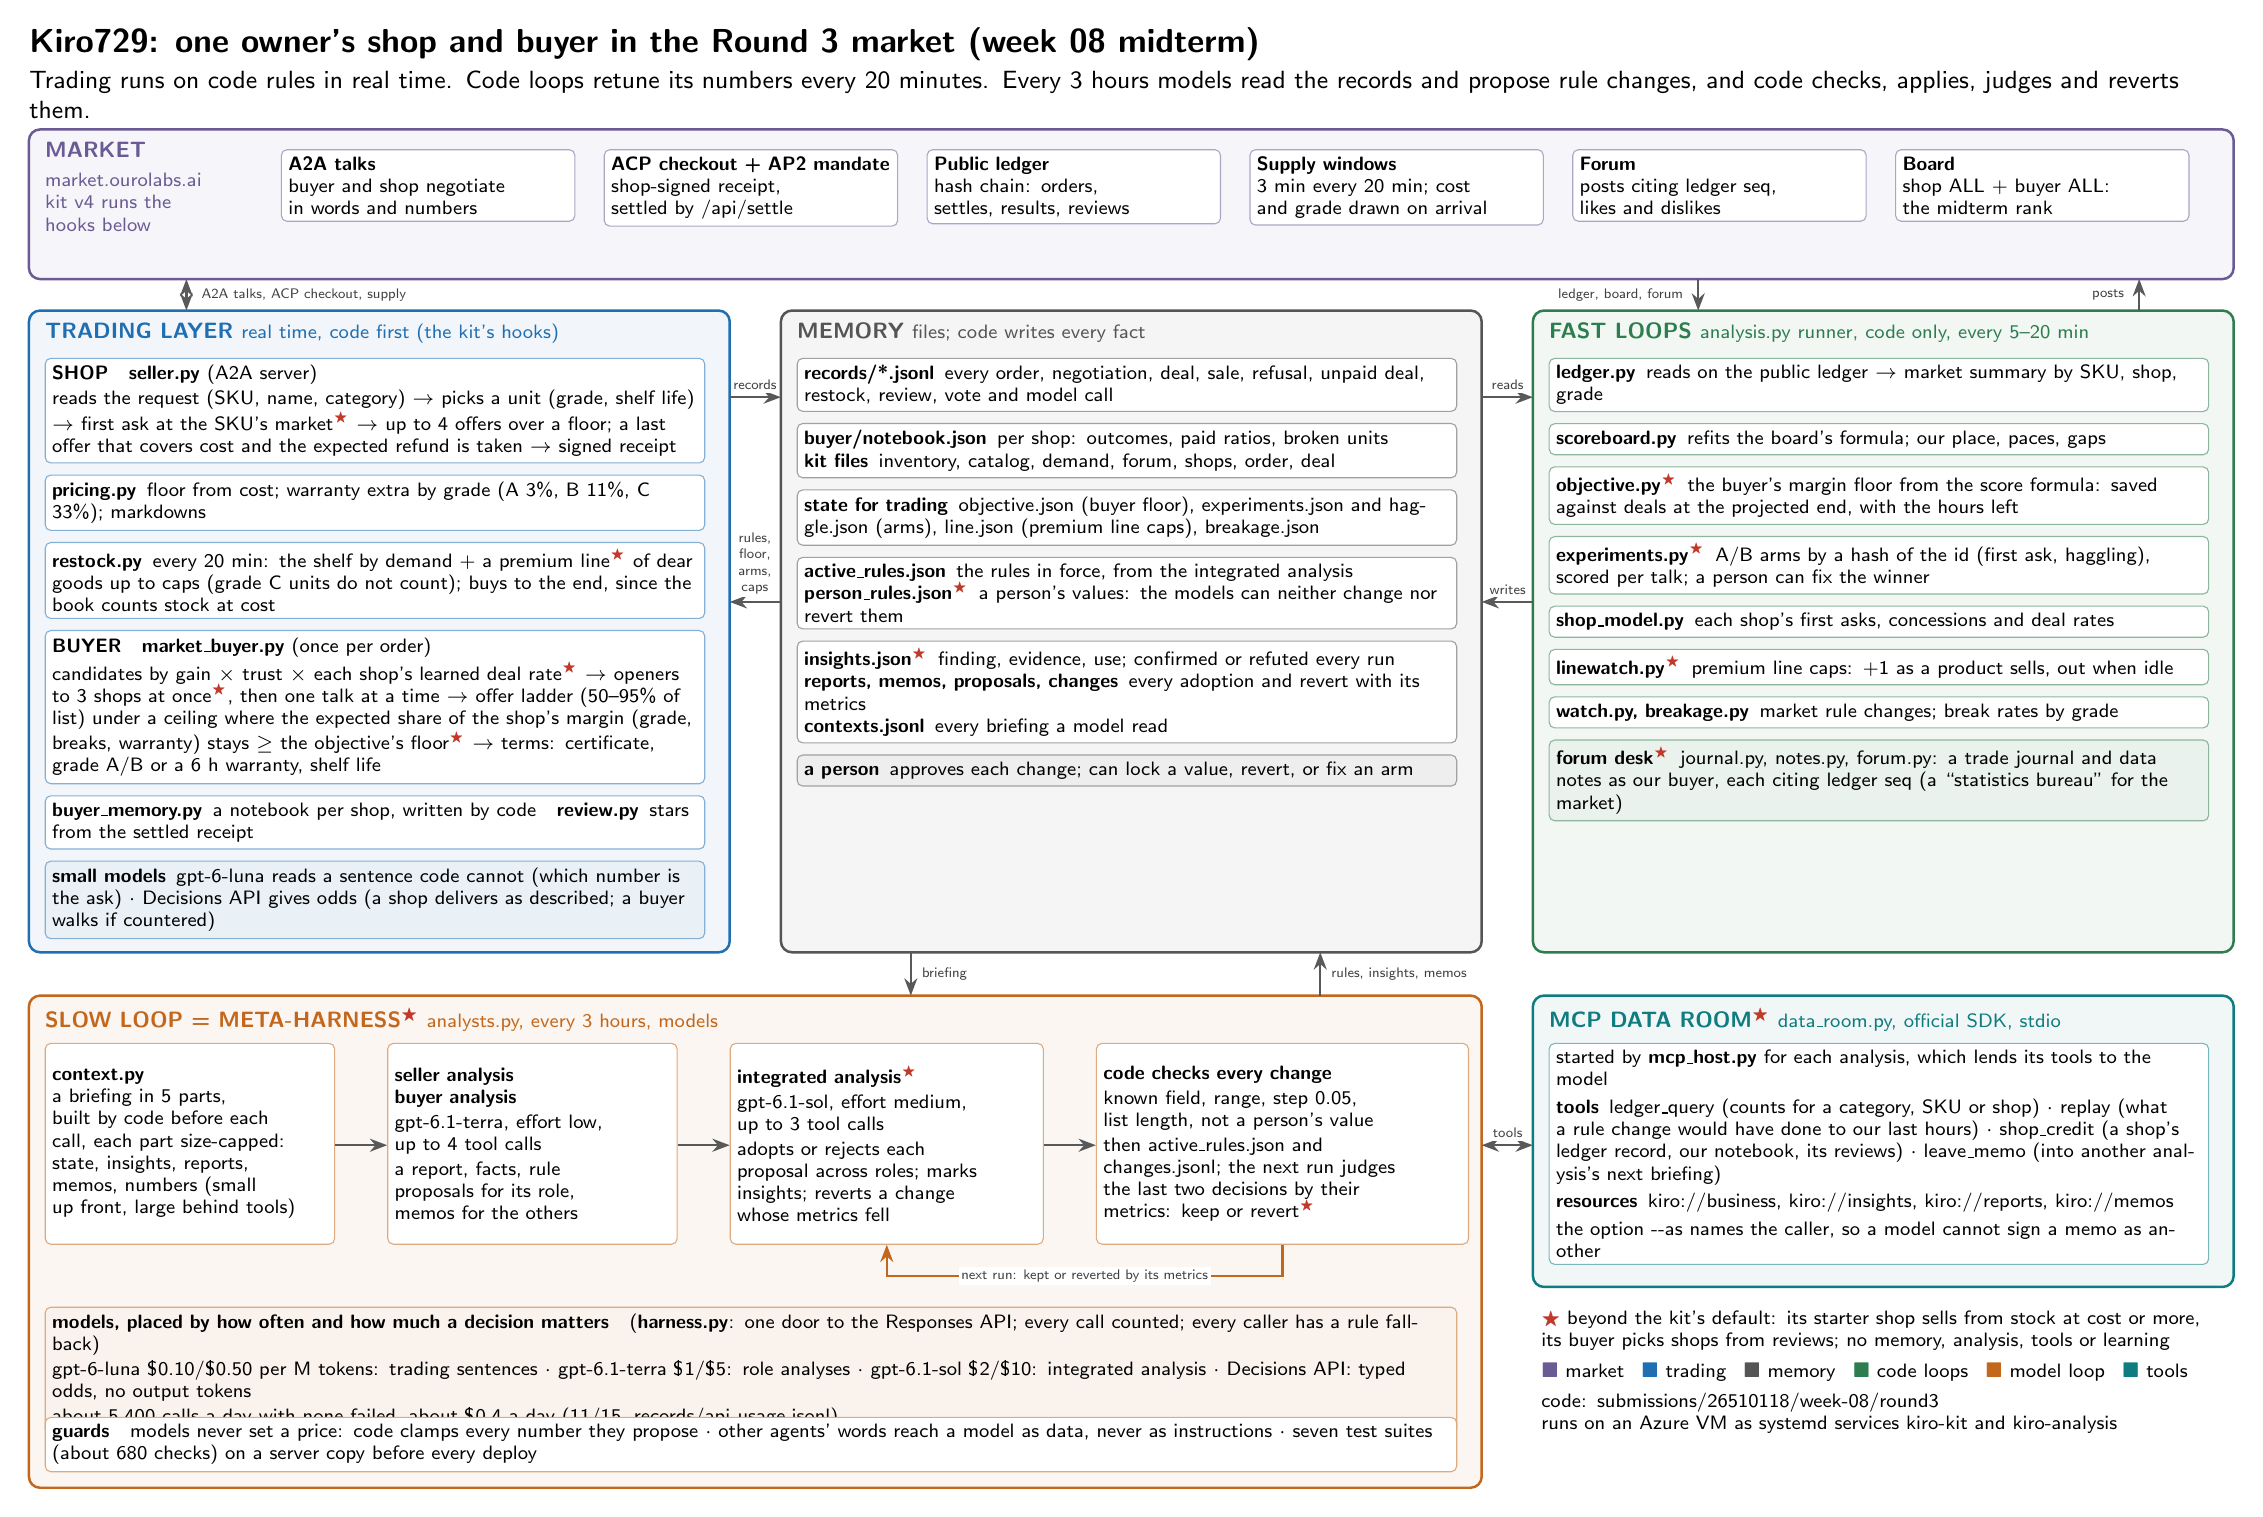
\begin{tikzpicture}[x=1cm,y=1cm]

% ------------------------------------------------------------------------- title
\node[anchor=north west, font=\large\bfseries, inner sep=0pt] at (0,19.5)
  {Kiro729: one owner's shop and buyer in the Round 3 market (week 08 midterm)};
\node[anchor=north west, font=\small, inner sep=0pt, text width=27.5cm] at (0,18.95)
  {Trading runs on code rules in real time. Code loops retune its numbers every 20 minutes. Every 3 hours
   models read the records and propose rule changes, and code checks, applies, judges and reverts them.};

% ------------------------------------------------------------------------- market
\draw[layer=mkt] (0,16.3) rectangle (28,18.2);
\node[head=mkt] at (0.2,18.05) {MARKET};
\node[anchor=north west, font=\scriptsize, text=mkt, align=left, inner sep=0pt] at (0.2,17.65)
  {market.ourolabs.ai\\ kit v4 runs the\\ hooks below};
\foreach \i/\t in {
  0/{\f{A2A talks}\\ buyer and shop negotiate\\ in words and numbers},
  1/{\f{ACP checkout + AP2 mandate}\\ shop-signed receipt,\\ settled by /api/settle},
  2/{\f{Public ledger}\\ hash chain: orders,\\ settles, results, reviews},
  3/{\f{Supply windows}\\ 3 min every 20 min; cost\\ and grade drawn on arrival},
  4/{\f{Forum}\\ posts citing ledger seq,\\ likes and dislikes},
  5/{\f{Board}\\ shop ALL + buyer ALL:\\ the midterm rank}} {
  \node[mod=mkt, text width=3.55cm] at ({3.2+\i*4.1},17.95) {\t};
}

% ------------------------------------------------------------------------- trading layer
\draw[layer=trd] (0,7.75) rectangle (8.9,15.9);
\node[head=trd] at (0.2,15.75) {TRADING LAYER \normalfont\scriptsize real time, code first (the kit's hooks)};
\node[col=trd] (shop) at (0.2,15.3) {%
  \f{SHOP}\quad\f{seller.py} (A2A server)\\[1pt]
  reads the request (SKU, name, category) $\rightarrow$ picks a unit (grade, shelf life)
  $\rightarrow$ first ask at the SKU's market\st{} $\rightarrow$ up to 4 offers over a floor; a last offer
  that covers cost and the expected refund is taken $\rightarrow$ signed receipt};
\node[col=trd, next=shop] (pricing) {%
  \f{pricing.py}\, floor from cost; warranty extra by grade (A 3\%, B 11\%, C 33\%); markdowns};
\node[col=trd, next=pricing] (restock) {%
  \f{restock.py}\, every 20 min: the shelf by demand + a premium line\st{} of dear goods up to
  caps (grade C units do not count); buys to the end, since the book counts stock at cost};
\node[col=trd, next=restock] (buyer) {%
  \f{BUYER}\quad\f{market\_buyer.py} (once per order)\\[1pt]
  candidates by gain $\times$ trust $\times$ each shop's learned deal rate\st{}
  $\rightarrow$ openers to 3 shops at once\st{}, then one talk at a time
  $\rightarrow$ offer ladder (50--95\% of list) under a ceiling where the expected share of the
  shop's margin (grade, breaks, warranty) stays $\geq$ the objective's floor\st{}
  $\rightarrow$ terms: certificate, grade A/B or a 6 h warranty, shelf life};
\node[col=trd, next=buyer] (bmem) {%
  \f{buyer\_memory.py}\, a notebook per shop, written by code\quad
  \f{review.py}\, stars from the settled receipt};
\node[col=trd, next=bmem, fill=trd!10] (small) {%
  \f{small models}\, gpt-6-luna reads a sentence code cannot (which number is the ask)
  $\cdot$ Decisions API gives odds (a shop delivers as described; a buyer walks if countered)};

% ------------------------------------------------------------------------- memory
\draw[layer=mem] (9.55,7.75) rectangle (18.45,15.9);
\node[head=mem] at (9.75,15.75) {MEMORY \normalfont\scriptsize files; code writes every fact};
\node[col=mem] (rec) at (9.75,15.3) {%
  \f{records/*.jsonl}\, every order, negotiation, deal, sale, refusal, unpaid deal, restock,
  review, vote and model call};
\node[col=mem, next=rec] (nb) {%
  \f{buyer/notebook.json}\, per shop: outcomes, paid ratios, broken units\\
  \f{kit files}\, inventory, catalog, demand, forum, shops, order, deal};
\node[col=mem, next=nb] (state) {%
  \f{state for trading}\, objective.json (buyer floor), experiments.json and haggle.json
  (arms), line.json (premium line caps), breakage.json};
\node[col=mem, next=state] (rules) {%
  \f{active\_rules.json}\, the rules in force, from the integrated analysis\\
  \f{person\_rules.json}\st{}\, a person's values: the models can neither change nor revert them};
\node[col=mem, next=rules] (know) {%
  \f{insights.json}\st{}\, finding, evidence, use; confirmed or refuted every run\\
  \f{reports, memos, proposals, changes}\, every adoption and revert with its metrics\\
  \f{contexts.jsonl}\, every briefing a model read};
\node[col=mem, next=know, fill=mem!10] (person) {%
  \f{a person}\, approves each change; can lock a value, revert, or fix an arm};

% ------------------------------------------------------------------------- fast loops
\draw[layer=fast] (19.1,7.75) rectangle (28,15.9);
\node[head=fast] at (19.3,15.75) {FAST LOOPS \normalfont\scriptsize analysis.py runner, code only, every 5--20 min};
\node[col=fast] (ledger) at (19.3,15.3) {%
  \f{ledger.py}\, reads on the public ledger $\rightarrow$ market summary by SKU, shop, grade};
\node[col=fast, next=ledger] (score) {%
  \f{scoreboard.py}\, refits the board's formula; our place, paces, gaps};
\node[col=fast, next=score] (obj) {%
  \f{objective.py}\st{}\, the buyer's margin floor from the score formula: saved
  against deals at the projected end, with the hours left};
\node[col=fast, next=obj] (exp) {%
  \f{experiments.py}\st{}\, A/B arms by a hash of the id (first ask, haggling), scored per
  talk; a person can fix the winner};
\node[col=fast, next=exp] (sm) {%
  \f{shop\_model.py}\, each shop's first asks, concessions and deal rates};
\node[col=fast, next=sm] (lw) {%
  \f{linewatch.py}\st{}\, premium line caps: +1 as a product sells, out when idle};
\node[col=fast, next=lw] (watch) {%
  \f{watch.py, breakage.py}\, market rule changes; break rates by grade};
\node[col=fast, next=watch, fill=fast!10] (desk) {%
  \f{forum desk}\st{}\, journal.py, notes.py, forum.py: a trade journal and data notes as our
  buyer, each citing ledger seq (a ``statistics bureau'' for the market)};

% ------------------------------------------------------------------------- slow loop (meta-harness)
\draw[layer=slow] (0,0.95) rectangle (18.45,7.2);
\node[head=slow] at (0.2,7.05) {SLOW LOOP = META-HARNESS\st{} \normalfont\scriptsize analysts.py, every 3 hours, models};
\node[mod=slow, text width=3.5cm, minimum height=2.55cm] (ctx) at (0.2,6.6) {%
  \f{context.py}\\ a briefing in 5 parts,\\ built by code before each\\ call, each part size-capped:\\ state, insights, reports,\\ memos, numbers (small\\ up front, large behind tools)};
\node[mod=slow, text width=3.5cm, minimum height=2.55cm] (role) at (4.55,6.6) {%
  \f{seller analysis}\\ \f{buyer analysis}\\[1pt] gpt-6.1-terra, effort low,\\ up to 4 tool calls\\[1pt] a report, facts, rule\\ proposals for its role,\\ memos for the others};
\node[mod=slow, text width=3.8cm, minimum height=2.55cm] (integ) at (8.9,6.6) {%
  \f{integrated analysis}\st{}\\[1pt] gpt-6.1-sol, effort medium,\\ up to 3 tool calls\\[1pt] adopts or rejects each\\ proposal across roles; marks\\ insights; reverts a change\\ whose metrics fell};
\node[mod=slow, text width=4.55cm, minimum height=2.55cm] (check) at (13.55,6.6) {%
  \f{code checks every change}\\[1pt] known field, range, step 0.05,\\ list length, not a person's value\\[1pt] then active\_rules.json and\\ changes.jsonl; the next run judges\\ the last two decisions by their\\ metrics: keep or revert\st{}};
\draw[flow] (ctx.east |- 0,5.3) -- (role.west |- 0,5.3);
\draw[flow] (role.east |- 0,5.3) -- (integ.west |- 0,5.3);
\draw[flow] (integ.east |- 0,5.3) -- (check.west |- 0,5.3);
\draw[flow, draw=slow] (check.south) -- ++(0,-0.4) -| node[lab, pos=0.25] {next run: kept or reverted by its metrics} (integ.south);
\node[mod=slow, text width=17.75cm, fill=slow!8] (models) at (0.2,3.25) {%
  \f{models, placed by how often and how much a decision matters}\quad (\f{harness.py}: one door to the
  Responses API; every call counted; every caller has a rule fallback)\\[1pt]
  gpt-6-luna \$0.10/\$0.50 per M tokens: trading sentences
  $\cdot$ gpt-6.1-terra \$1/\$5: role analyses
  $\cdot$ gpt-6.1-sol \$2/\$10: integrated analysis
  $\cdot$ Decisions API: typed odds, no output tokens\\[1pt]
  about 5,400 calls a day with none failed, about \$0.4 a day (11/15, records/api\_usage.jsonl)};
\node[mod=slow, text width=17.75cm] (guards) at (0.2,1.85) {%
  \f{guards}\quad models never set a price: code clamps every number they propose
  $\cdot$ other agents' words reach a model as data, never as instructions
  $\cdot$ seven test suites (about 680 checks) on a server copy before every deploy};

% ------------------------------------------------------------------------- MCP data room
\draw[layer=mcp] (19.1,3.5) rectangle (28,7.2);
\node[head=mcp] at (19.3,7.05) {MCP DATA ROOM\st{} \normalfont\scriptsize data\_room.py, official SDK, stdio};
\node[col=mcp] (room) at (19.3,6.6) {%
  started by \f{mcp\_host.py} for each analysis, which lends its tools to the model\\[2pt]
  \f{tools}\, ledger\_query (counts for a category, SKU or shop) $\cdot$ replay (what a rule change
  would have done to our last hours) $\cdot$ shop\_credit (a shop's ledger record, our notebook,
  its reviews) $\cdot$ leave\_memo (into another analysis's next briefing)\\[2pt]
  \f{resources}\, kiro://business, kiro://insights, kiro://reports, kiro://memos\\[2pt]
  the option \mbox{-{}-as} names the caller, so a model cannot sign a memo as another};

% ------------------------------------------------------------------------- legend
\node[anchor=north west, font=\scriptsize, align=left, inner sep=0pt, text width=8.6cm] at (19.2,3.2) {%
  \textcolor{star}{$\bigstar$} beyond the kit's default: its starter shop sells from stock at
  cost or more, its buyer picks shops from reviews; no memory, analysis, tools or learning\\[3pt]
  \textcolor{mkt}{$\blacksquare$} market \enspace \textcolor{trd}{$\blacksquare$} trading \enspace
  \textcolor{mem}{$\blacksquare$} memory \enspace \textcolor{fast}{$\blacksquare$} code loops \enspace
  \textcolor{slow}{$\blacksquare$} model loop \enspace \textcolor{mcp}{$\blacksquare$} tools\\[3pt]
  code: submissions/26510118/week-08/round3 \\
  runs on an Azure VM as systemd services kiro-kit and kiro-analysis};

% ------------------------------------------------------------------------- arrows between layers
\draw[both] (2.0,16.3) -- (2.0,15.9);
\node[lab, anchor=west] at (2.15,16.1) {A2A talks, ACP checkout, supply};
\draw[flow] (21.2,16.3) -- (21.2,15.9);
\node[lab, anchor=east] at (21.05,16.1) {ledger, board, forum};
\draw[flow] (26.8,15.9) -- (26.8,16.3);
\node[lab, anchor=east] at (26.65,16.1) {posts};
\draw[flow] (8.9,14.8) -- (9.55,14.8);
\node[lab, anchor=south] at (9.22,14.85) {records};
\draw[flow] (9.55,12.2) -- (8.9,12.2);
\node[lab, anchor=south] at (9.22,12.25) {rules,\\floor,\\arms,\\caps};
\draw[flow] (18.45,14.8) -- (19.1,14.8);
\node[lab, anchor=south] at (18.78,14.85) {reads};
\draw[flow] (19.1,12.2) -- (18.45,12.2);
\node[lab, anchor=south] at (18.78,12.25) {writes};
\draw[flow] (11.2,7.75) -- (11.2,7.2);
\node[lab, anchor=west] at (11.3,7.47) {briefing};
\draw[flow] (16.4,7.2) -- (16.4,7.75);
\node[lab, anchor=west] at (16.5,7.47) {rules, insights, memos};
\draw[both] (18.45,5.3) -- (19.1,5.3);
\node[lab, anchor=south] at (18.78,5.35) {tools};

\end{tikzpicture}
\end{document}
